\subsection{Generalized Suppressed Fuzzy C-Means}
\label{subsec:fuzzycmeansresults}

\begin{figure}[ht!]
    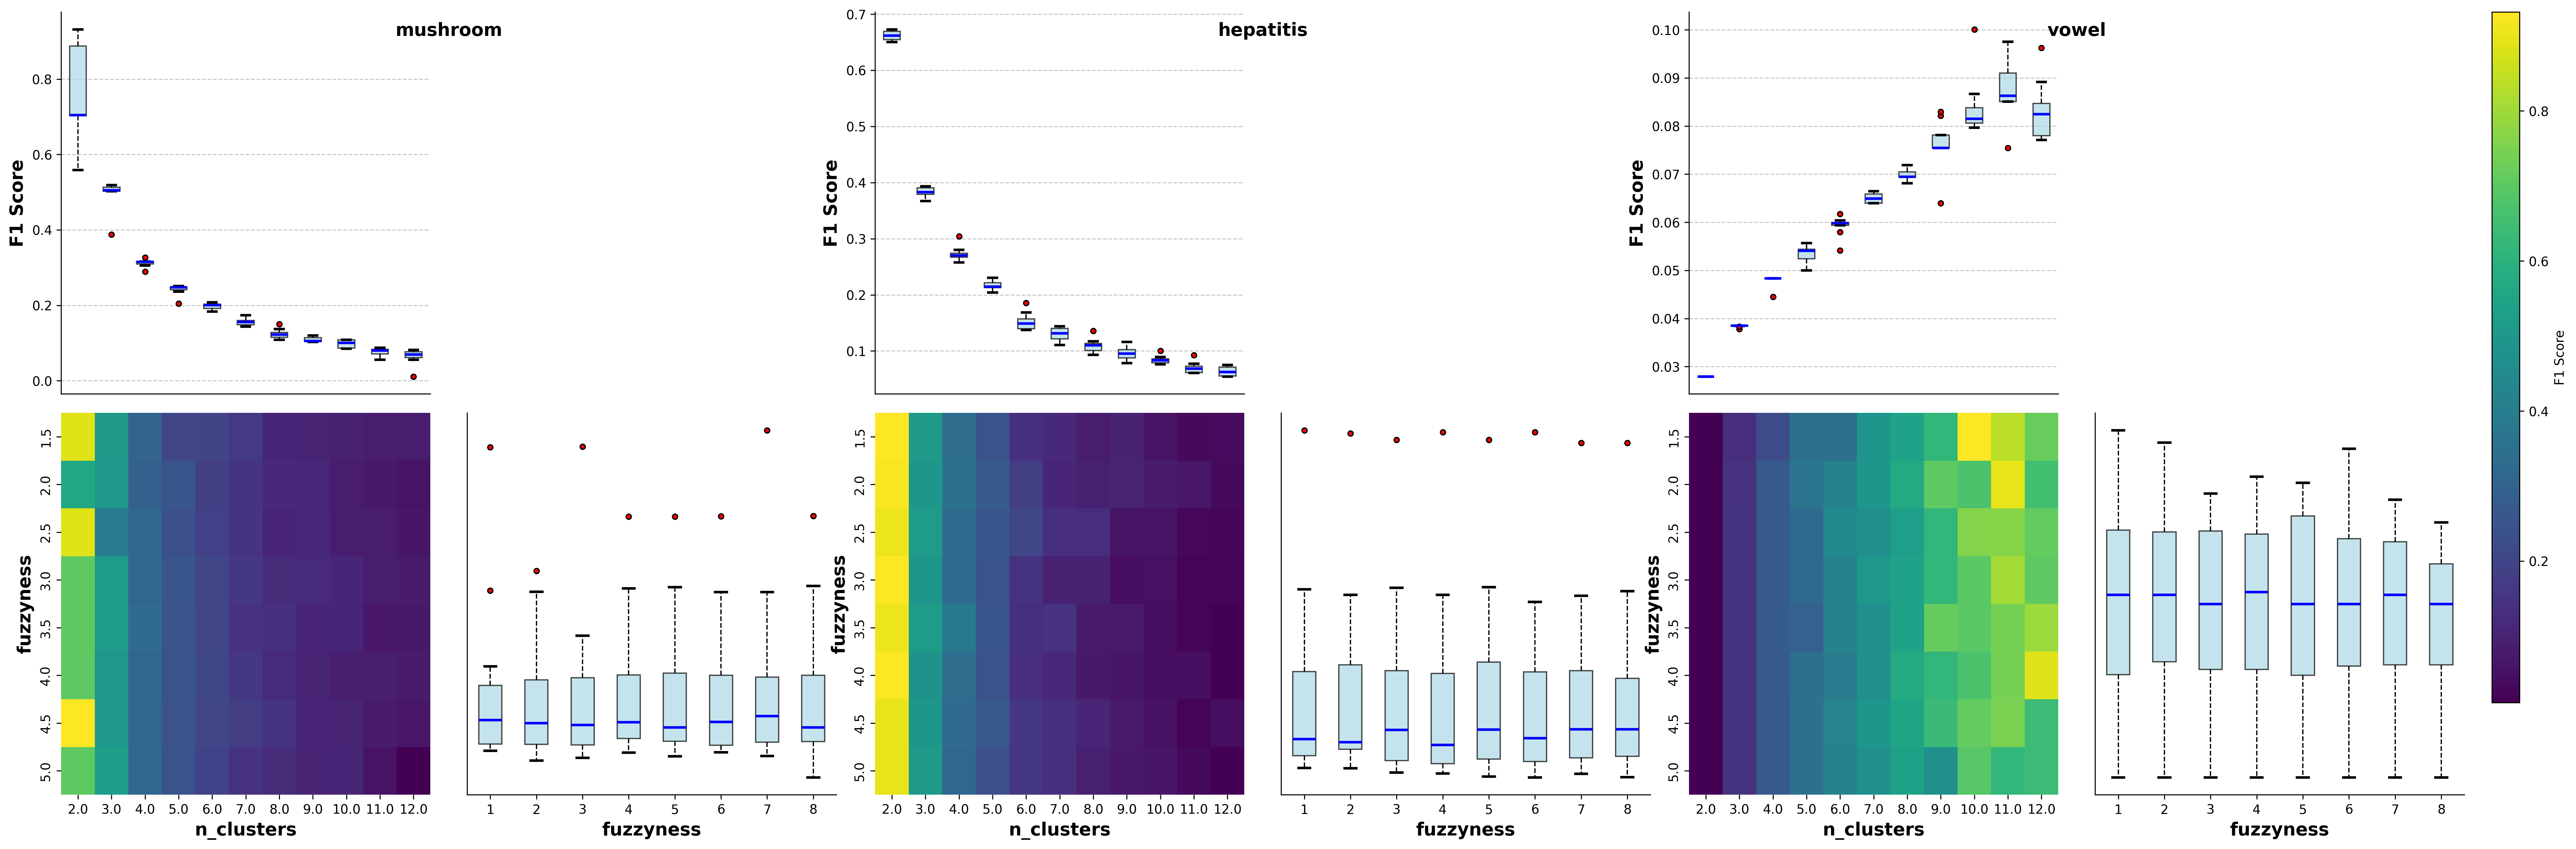
\includegraphics[width=0.5\textwidth]{figures/interactions_fuzzy_cmeans.png}
    \caption{Parameter interactions for gs-FCM}
    \label{fig:interactions_gsfcm}
\end{figure}


Figure~\ref{fig:interactions_gsfcm} presents the interaction effects between the key parameters of the gs-FCM clustering algorithm: the number of clusters ($n\_clusters$) and the fuzziness coefficient, across three datasets: \textit{hepatitis}, \textit{mushroom}, and \textit{vowel}.

The \textit{hepatitis} dataset shows optimal performance with fewer clusters and lower fuzziness values (closer to 1.5), suggesting that simpler, more crisp clustering is appropriate. The \textit{mushroom} dataset demonstrates robustness across parameter combinations, maintaining high F1 scores regardless of parameter settings. In contrast, the \textit{vowel} dataset benefits from higher complexity, achieving better performance with larger $n\_clusters$ and higher fuzziness values.

These results highlight the importance of dataset-specific parameter tuning in gs-FCM clustering, as each dataset exhibits distinct optimal configurations based on its underlying characteristics.

